\documentclass[tikz,border=8pt]{standalone}
\usetikzlibrary{positioning,fit}
\begin{document}
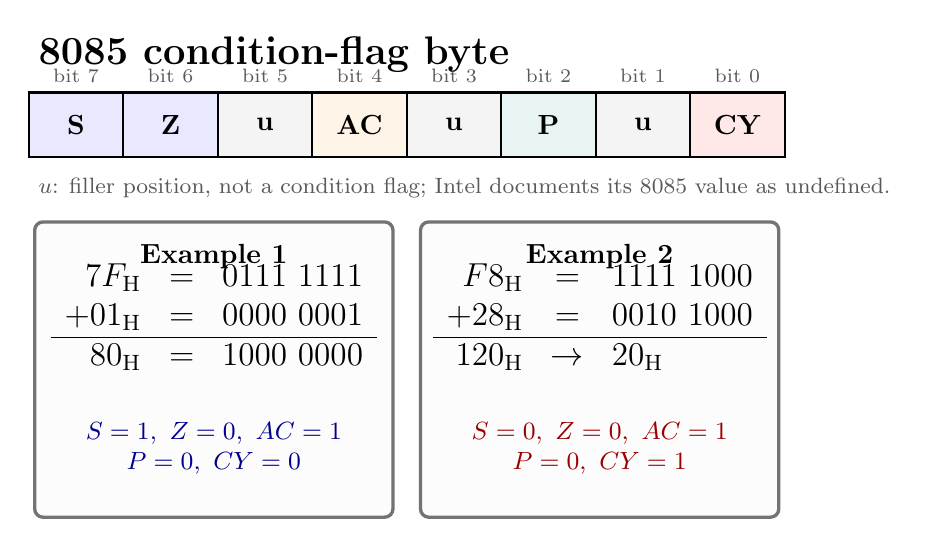
\begin{tikzpicture}[font=\sffamily]
  \node[font=\bfseries\Large,anchor=west] at (0,3.25) {8085 condition-flag byte};
  \foreach \i/\bit/\name/\col in {
    0/7/S/blue,1/6/Z/blue,2/5/u/gray,3/4/AC/orange,
    4/3/u/gray,5/2/P/teal,6/1/u/gray,7/0/CY/red}{
    \draw[thick,fill=\col!9] (1.2*\i,1.95) rectangle ++(1.2,.82);
    \node[font=\bfseries] at (1.2*\i+.6,2.36) {\name};
    \node[font=\scriptsize,text=black!65] at (1.2*\i+.6,2.98) {bit \bit};
  }
  \node[font=\footnotesize,text=black!65,anchor=west] at (0,1.55) {$u$: filler position, not a condition flag; Intel documents its 8085 value as undefined.};

  \node[draw=black!55,rounded corners=3pt,very thick,minimum width=4.55cm,minimum height=3.75cm,fill=black!1] (ex1) at (2.35,-.75) {};
  \node[font=\bfseries,anchor=north] at ([yshift=-.18cm]ex1.north) {Example 1};
  \node[font=\large] at (2.35,-.1) {$\begin{array}{rcl}7F_{\rm H}&=&0111\ 1111\\+01_{\rm H}&=&0000\ 0001\\\hline 80_{\rm H}&=&1000\ 0000\end{array}$};
  \node[font=\small,align=center,text=blue!55!black] at (2.35,-1.75) {$S=1,\ Z=0,\ AC=1$\\$P=0,\ CY=0$};

  \node[draw=black!55,rounded corners=3pt,very thick,minimum width=4.55cm,minimum height=3.75cm,fill=black!1] (ex2) at (7.25,-.75) {};
  \node[font=\bfseries,anchor=north] at ([yshift=-.18cm]ex2.north) {Example 2};
  \node[font=\large] at (7.25,-.1) {$\begin{array}{rcl}F8_{\rm H}&=&1111\ 1000\\+28_{\rm H}&=&0010\ 1000\\\hline 120_{\rm H}&\rightarrow&20_{\rm H}\end{array}$};
  \node[font=\small,align=center,text=red!60!black] at (7.25,-1.75) {$S=0,\ Z=0,\ AC=1$\\$P=0,\ CY=1$};
\end{tikzpicture}
\end{document}
